\chapter{Architecure and Design}
\label{chapter:architecture}

Before we reach the point of discussing a new future-proof, modern architecture and design of Tribler, the evolution of the Tribler architecture  throughout the last 10 years will be elaborated. Understanding the past decisions regarding architecture and design, will help us to shed light on the question why Tribler has accumulated such an amount of technical debt.\\\\
According to GitHub, Tribler has a total of 44 unique contributors so far. This list is most likely not complete since some work of missing contributors might have been finished by another member of the Tribler team. Searching for \emph{Tribler} in the TU Delft repository, results in a total of 66 hits of which 35 results are contributions in the form of a MSc or BSc thesis.\\\\
The remaining of this chapter will present a historical description of the evolution of Tribler. Next, a new architecture will be proposed and discussed in detail. This will lay the foundations for the next decade of research in the area of peer-to-peer network and anonymity.

\section{Tribler: A social-based peer-to-peer system}
Tribler started out as fork from \emph{Another BitTorrent Client} (ABC), an improved BitTorrent client. ABC is based on \emph{BitTornado} which extended from the \emph{BitTorrent} core system, written by Bram Cohen. In the current code base of Tribler, various references to ABC can be found, mostly notable in the naming of files, variables and classes.\\\\
In 2007, the first major research paper was published, describing Tribler as a social-based peer-to-peer system\cite{pouwelse2008tribler}. The key idea is that social connections between peers in a decentralized network can be exploited to increase usability and performance of the network. This is based on the idea that peers belonging to a social group are not likely to steal (free-ride) bandwidth from each other. The system architecture of the system is visible in Figure \ref{fig:tribler-architecture-2008}. In the remainder of this Section, the most important components of the architecture as described in \cite{pouwelse2008tribler} will be explained in more detail.

\begin{figure}[t]
	\centering
	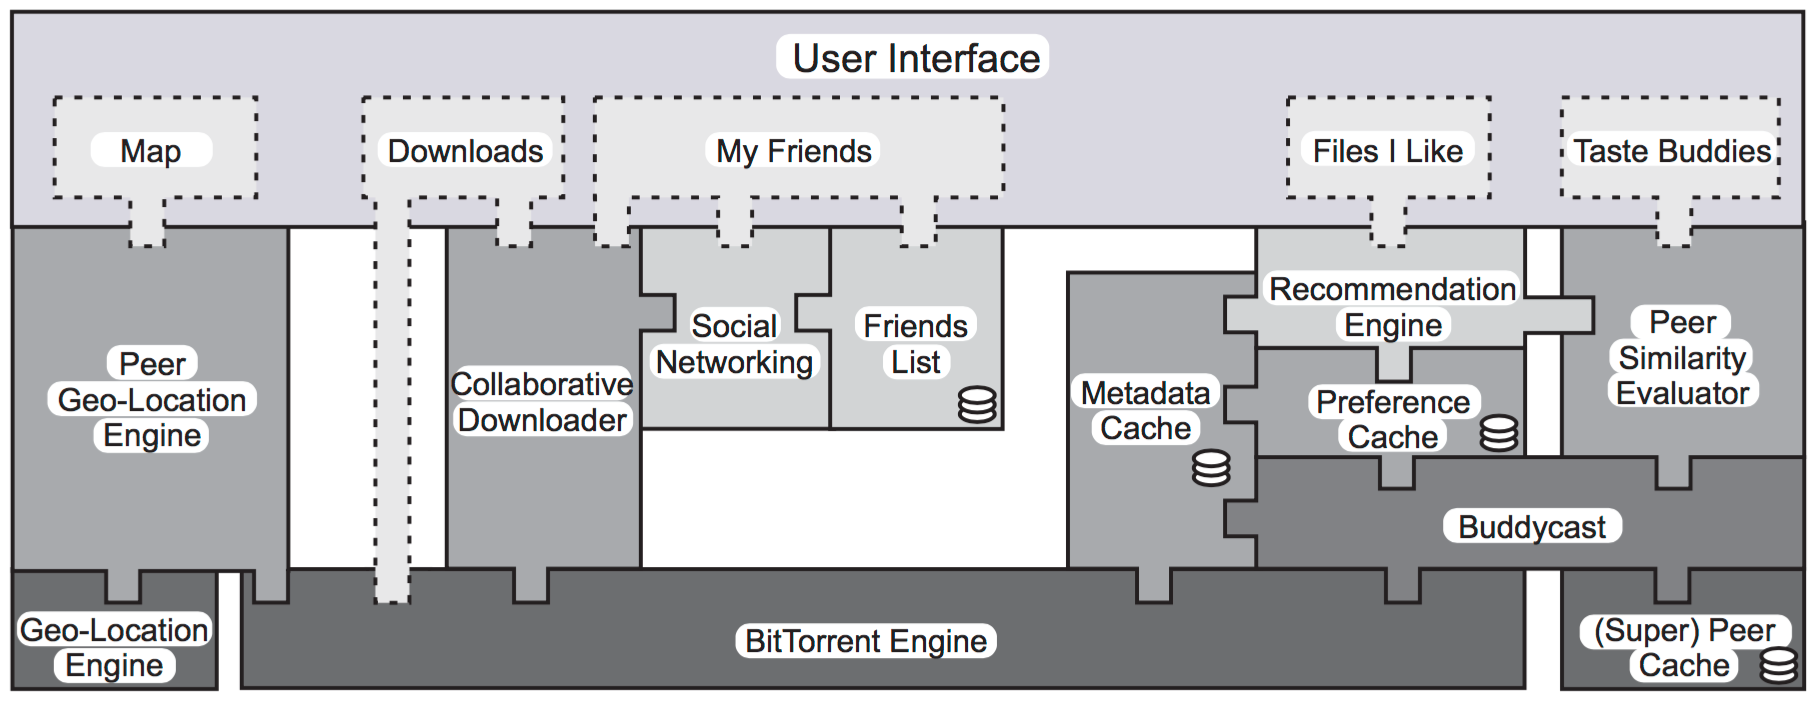
\includegraphics[width=0.9\columnwidth]{images/tribler_architecture_2007}
	\caption{The system architecture as described in \cite{pouwelse2008tribler}.}
	\label{fig:tribler-architecture-2008}
\end{figure}

\subsection{Collaborative Downloads}
The BitTorrent engine allows the mechanism to download and seed torrent files using a BitTorrent-compatible protocol. In addition, the module allows usage of the \emph{collaborative downloader} module which significantly increases download speed by exploiting idle upload capacity of online friends.\\\\
The protocol to facilitate collaborative downloads is called \emph{2Fast} and the idea is that a user invokes the help of friends to increase download speed of his files. The protocol uses social groups where members who trust each other collaborate to improve their download performance. Peers that are participating in a social group are either \emph{collectors} or \emph{helpers}. A collector is a peer that is interested in obtaining a complete copy of a particular file. A helper is a peer that is recruited by a collector to help downloading that file.

\subsection{Peer Geo-Location Engine}
The \emph{Peer Geo-Location Engine} is an engine built on top of a module that enables geographical lookup of IP addresses (\emph{http://hostip.info}). When a peer downloads a file, peers in the download swarm are displayed on a map in the user interface.

\subsection{Content Discovery and Recommendation}
The \emph{BuddyCast} algorithm is designed to make recommendations and to enable peer and content discovery. BuddyCast is an epidemic protocol which works as follows: each peer in the network maintains a number of taste buddies with their preference lists and a numer of random peers without any information about their preferences. Periodically, an \emph{exploration} or \emph{exploitation} step is performed. When an exploration is executed, the peer connects to one of its taste buddies. The peer connects to a random peer if an exploitation step is performed. When the connection is successful, a \emph{BuddyCast} message is exchanged.\\\\
A Buddycast message contains the identities of a number of taste buddies along with their top-10 preference lists, a number of random (and fresh, see below) peers, and the top-50 preferences of the sending peer. The age of each peer is included in the message to help others know the freshness of peers. After the BuddyCast messages are exchanged, the received information is stored in the local database of each peer. To limit redundant messages, each peer maintains a list of recently contacted peers.

\section{Shaping the next generation of internet TV}
In 2008, the European Union funded the P2P-Next research effort\cite{p2pnextpressrelease}. The project was active starting from 2008 to 2012 and planned to conduct a large-scale technical trial of new media applications running on a wide range of consumer devices, using peer-to-peer technologies. Tribler has been the main subject of research during the P2P-Next project by TU Delft. This Section will explain the conducted research and architectural evolution during the P2P-Next project.

\subsection{Libswift}

% http://delivery.acm.org/10.1145/2080000/2072433/p739-zeilemaker.pdf?ip=145.94.5.138&id=2072433&acc=ACTIVE%20SERVICE&key=0C390721DC3021FF%2E512956D6C5F075DE%2E4D4702B0C3E38B35%2E4D4702B0C3E38B35&CFID=816981133&CFTOKEN=23604061&__acm__=1469268778_0dc54a276c6ce7abce65547df9722e66

% TODO explain threading model